\documentclass[12pt,a4paper]{article}

\usepackage[utf8]{inputenc}
\usepackage[english]{babel}
\usepackage{amsmath}
\usepackage{amsfonts}
\usepackage{amssymb}
\usepackage{graphicx}
\usepackage{cite}
\usepackage{hyperref}
\usepackage[left=2cm,right=2cm,top=2cm,bottom=2cm]{geometry}
\usepackage{booktabs}
\usepackage{xcolor,colortbl}
\usepackage{pstricks}
\usepackage{eurosym} 
\usepackage{longtable}
\usepackage{blindtext}
\usepackage{fancyhdr}
\usepackage{lastpage}
\usepackage{pdfpages}
\usepackage{tabularx} 
\usepackage{transparent}
\usepackage{array}
\usepackage{etoolbox}
\usepackage{float}
\usepackage{lscape}

\begin{document}


\section{Communications logictic}

\subsection{Characteristics of the constellation}
\paragraph{}In order to define the logistics of the communications, it is needed to take into account the different characteristics of the constellation and the satellites that are part of it.
\begin{itemize}
\item The constellation is formed by a series of polar, or near polar, orbital planes, covering the whole world.
\item Satellites in neightbouring planes move in the same direction (from north to south, or from south to north), creating two hemispheres. In one, satellites move from the south towards the north, and in the other satellites move from the north towards the south.
\item Each satellite can communicate with a potential client upwards, with a ground station downwards, with the next and the previous satellites in the same orbital plane, and with a satellite in eachneightbouring plane. If the adjacent plane moves in the opposite direction, the satellites will not communicate between them.
\item Each communication link is independent, therefore, a satellite can communicate across the orbital plane while at the same time is communicating across planes.
\item Moreover, each communication link has different channels to communicate, resulting in different communications happening in the same direction at the same time.
\item The constellation can be used to communicate two nodes, which can be either satellites or ground stations.
\end{itemize}

\begin{figure}[H]
\centering
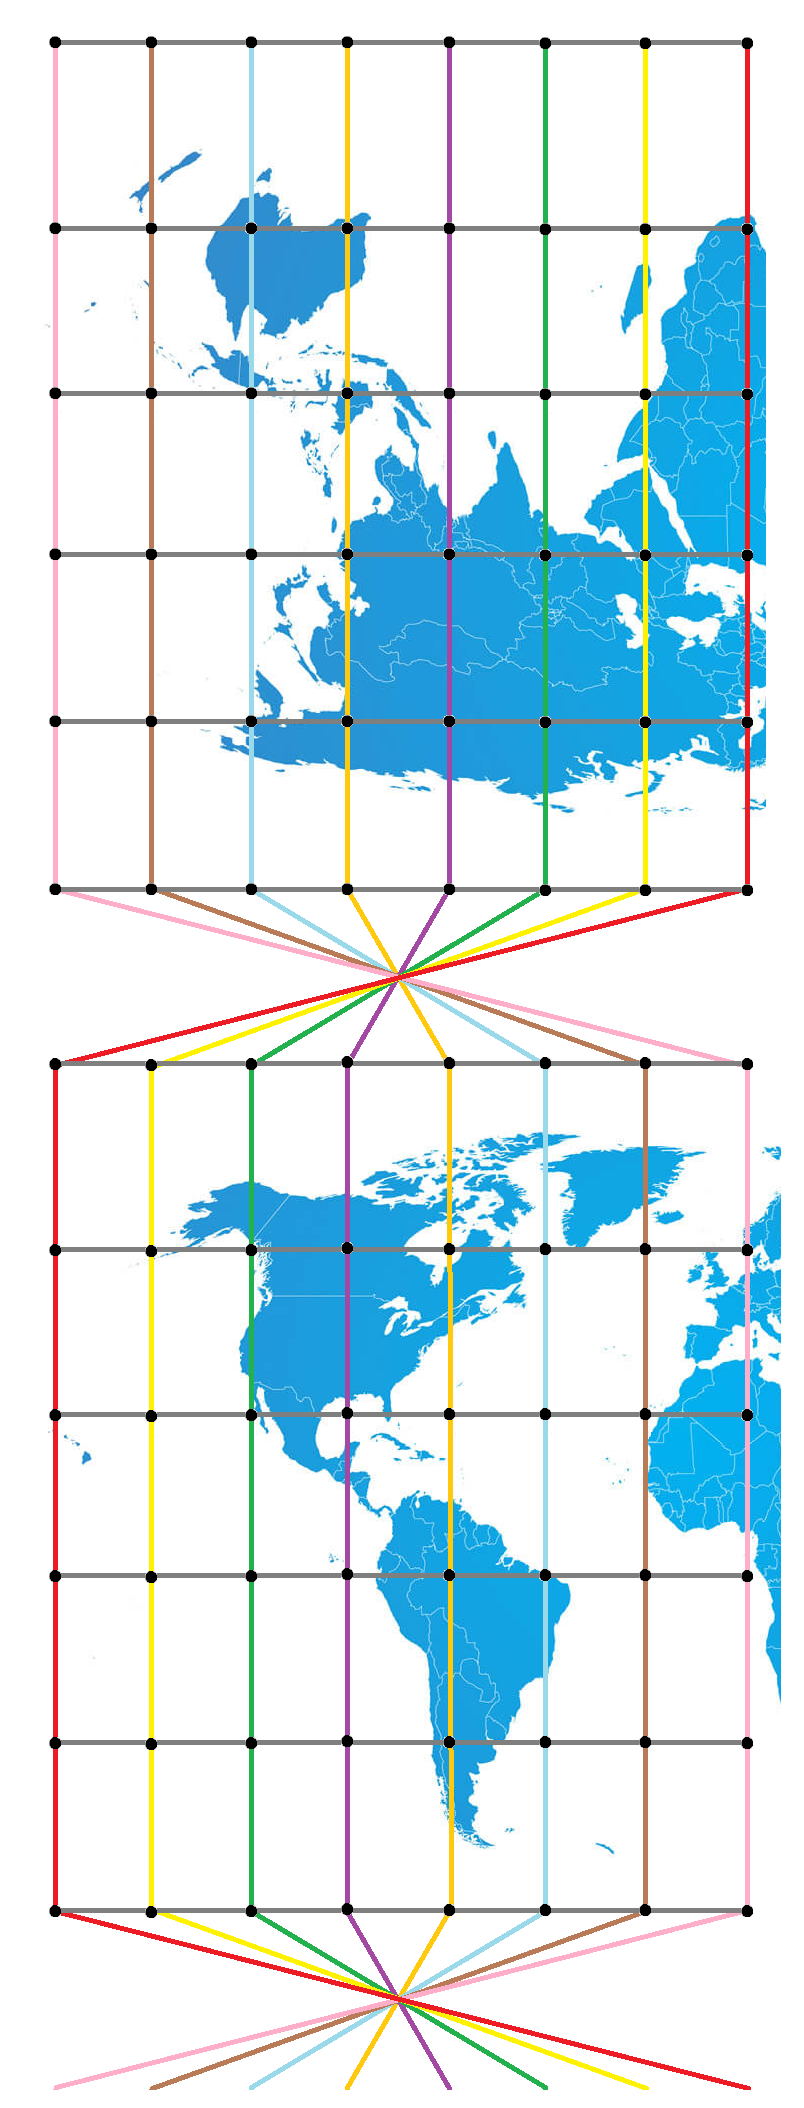
\includegraphics[scale=0.3]{network.png}
\caption[Shceme of the constellation]{Scheme of the constellation. Black dots are satellites. Color lines are communication links in the same orbital plane. Grey lines are links between orbital planes.}
\label{Scheme of the constellation}
\end{figure}

\subsection{Logistics}
\paragraph{}In order to communicate properly within the network, the data to deliver will have a introductory sequence indicating its origin and its destination. Each satellite will have a map of the constellation, with the variation of the positions of each satellite and ground station over time. Before transmitting the data, a satellite will emit a signal to the following satellite to check its status and to indicate the intention of using any of the satellite links. If the satellite is active and it is avaiable for communications, it will return a signal to indicate the avaiability. 

\paragraph{}The path that will follow the data will be the following: in the network map, the data will first travel along the orbit upon reaching the closest satellite at the destination latitude, then, it will change orbital planes upon reaching the closest satellite to the destination.

\paragraph{}In case a satellite is inactive, it can not return a signal, and the emitting satellite will not transmit to that satellite and will find and alternative route. If the satellite is active, but the intended route for the emitting satellite is alredy being used in all of the channels, it will return a signal saying that is occupied.

\paragraph{}When a satellite cannot transmit in the regular path, it will use the alternate path. The alternate path consists in first transmitting in the different orbital planes upon reaching the satellite closest to the target longitude, and then trveling along the orbital plane upon reaching the closest satellite to the target. If the alternate path is also unable of being used, the satellite will try to use the regular path once again, and will alternate with the two paths until one of them is able. Meanwhile, the satellite will store the data.

\paragraph{}From all the channels in each link, one of them will be reserved. This is the channel that will be used for the company's ground station to check the status of the constellation and giving orders to the satellites of the constellation.


\end{document}